\title{Solving a Cosserat Rod Boundary Value Problem}
\author{John Till}
\date{}

\documentclass[12pt]{article}

\usepackage[a4paper, margin=0.75in]{geometry}
\usepackage[colorlinks=true,urlcolor=blue]{hyperref}
\usepackage{amsmath,amssymb}
\usepackage{graphicx}

\usepackage{xcolor}
\definecolor{OffWhite}{rgb}{0.93,0.93,0.93}
\definecolor{QtCommentColor}{rgb}{0,0.5,0}
\definecolor{QtKeywordColor}{rgb}{0.5,0.5,0}
\definecolor{QtPurpleColor}{rgb}{0.5,0,0.5}
\definecolor{QtGlobal}{rgb}{0.808,0.361,0}
\definecolor{QtFunctionColor}{rgb}{0,0.404,0.486}

\usepackage[T1]{fontenc} %for upquotes in listings
\usepackage{textcomp} %for upquotes in listings
\usepackage{listings}
\lstset{
		language=C++,
		escapeinside={!-}{-!},
		upquote=true,
		%
		otherkeywords={Vector3d, DiagonalMatrix, VectorXd, Matrix3d, Map, MatrixXd, Vector6d,
									UnitX, pow, inverse, transpose, segment, data, UnitZ, cross, hat,
									Zero, Identity, UnitY, cosseratRodOde, ode4, cols, row, main, shootingFunction,
									block, rotation_error, solveLevenbergMarquardt, plot},
    morekeywords=[2]{Vector3d, DiagonalMatrix, VectorXd, Matrix3d, Map, MatrixXd, Vector6d},
		morekeywords=[3]{UnitX, UnitZ, pow, inverse, transpose, segment, data, cross, hat,
		                 Zero, Identity, UnitY, cosseratRodOde, ode4, cols, row, main, shootingFunction,
										 block, rotation_error, solveLevenbergMarquardt, plot},
    %
		frame = single,
		rulecolor=\color{black},
    tabsize=4, % tab space width
    showstringspaces=false, % don't mark spaces in strings
		%
		basicstyle=\footnotesize,%\color{QtIdentifier},
		backgroundcolor=\color{OffWhite},
    commentstyle=\color{QtCommentColor}, % comment color
    keywordstyle=\color{QtKeywordColor}, % keyword color
		keywordstyle=[2]{\color{QtPurpleColor}},
		keywordstyle=[3]{\color{QtFunctionColor}},
    stringstyle=\color{QtCommentColor} % string color
}

\begin{document}

\makeatletter
\renewcommand{\@maketitle}{
\newpage
\null
\vskip 2em
\begin{center}
{\LARGE \@title \par}
\end{center}
\par
} \makeatother

\maketitle

In the last chapter we solved a Cosserat rod initial value problem where $\boldsymbol{p}(0)$, $\boldsymbol{R}(0)$, $\boldsymbol{n}(0)$, and $\boldsymbol{m}(0)$ are known. However, in most applications we won't have a 6-dof force sensor attached at the base to measure $\boldsymbol{n}(0)$ and $\boldsymbol{m}(0)$. More commonly we know information at either end, for example if a robot uses two grippers to hold both ends of the rod, then we know $\boldsymbol{p}(0)$, $\boldsymbol{R}(0)$, $\boldsymbol{p}(L)$, and $\boldsymbol{R}(L)$. We can still solve such a problem, known as a boundary value problem (BVP), but the process is more complicated.

Since we're going to be referring to the boundary conditions (BCs) in several functions, we declare them as global variables:
\begin{lstlisting}
//Boundary conditions
const Vector3d p0 = Vector3d::Zero();
const Matrix3d R0 = Matrix3d::Identity();
const Vector3d pL = Vector3d(0, -0.1*L, 0.8*L);
const Matrix3d RL = Matrix3d::Identity();
\end{lstlisting}
There's nothing too exciting here; Vector3d has nice constructor which allows us to set each element. Now we've specified the pose (position and orientation) at both ends of the rod.

There are various methods of numerically solving BVPs, but since our problem is one-dimensional and we eventually want the solution process to be fast, we'll rely on the shooting method. There are two parts to a shooting method, an \emph{objective function} and a solver. The objective function input is a guess for the unknown state variables at one of the boundary, then the ODE is integrated to determine how badly the boundary conditions at the other end are violated. The solver minimizes this error violation, hopefully driving it to zero by some algorithm such as Newton-Raphson or Levenberg-Marquardt. The \emph{numerical shooting method} is a well known approach with explanations readily available online, so I won't go into more detail here.

We write the \emph{objective function} in C++ which takes the guessed base wrench (force and moment) as an input, then numerically integrates the rod to find the error in the pose (position and orientation) at the end:
\begin{lstlisting}
static MatrixXd Y; //Declare Y global for shooting and visualization
VectorXd shootingFunction(VectorXd guess){
    VectorXd y0(18);
    y0 << p0, Map<VectorXd>(Matrix3d(R0).data(), 9), guess;

    //Numerically integrate the Cosserat rod equations
    Y = ode4<cosseratRodOde>(y0, L);

    //Calculate the pose (position and orientation) error at the far end
    Vector3d pL_shooting = Y.block<3,1>(0, Y.cols()-1);
    Matrix3d RL_shooting = Map<Matrix3d>(Y.block<9,1>(3, Y.cols()-1).data());

    Vector6d distal_error;
    distal_error << pL - pL_shooting, rotation_error(RL,RL_shooting);

    return distal_error;
}
\end{lstlisting}
We set the initial state including the guessed part, integrate the rod as an IVP, then compare the values of $\boldsymbol{p}(L)$ and $\boldsymbol{R}(L)$ which we found by ``shooting'' with the actual values of $\boldsymbol{p}(L)$ and $\boldsymbol{R}(L)$. The position error calculation is straightforward, but comparing the rotation matrices requires a bit more effort. A rotation is a 3x3 matrix, but there aren't 9 independent error components between two rotations because each rotation already has its own set of constraints that $\boldsymbol{R}^T \boldsymbol{R} = \boldsymbol{I}$ and that the determinant of $\boldsymbol{R}$ is 1. This is why the ``rotation\_error'' function returns a 3x1 vector expressing the error between the rotation matrices. Specifically, it calculates
\begin{align*}
err = \left( \log (\boldsymbol{R}_1 \boldsymbol{R}_2^T) \right)^\vee
\end{align*}
The $(\cdot)^\vee$ operator is the inverse of the hat $\widehat{\cdot}$ operator, and the ``log'' is a matrix logarithm.

Now we can solve the BVP by using a solver on the objective function. \emph{Convex optimization} routines are defined in ``convexoptimization.h'', and we make a call to one of these algorithms:
\begin{lstlisting}
int main(int, char**){
    Vector6d init_guess = Vector6d::Zero();

    //Solve with shooting method
    VectorXd wrench_soln = solveLevenbergMarquardt<shootingFunction>(init_guess);
\end{lstlisting}
The solver requires an initial guess, which we trivially supply as $\begin{bmatrix} 0 & 0 & 0 & 0 & 0 & 0\end{bmatrix}^T$. The method used to find the correct base reaction wrench is the \emph{Levenberg-Marquardt algorithm}, but while considering the rod BVP we can regard it as a blackbox solver. Now we have solved the problem and we can plot the result.
\begin{figure}[h]
	\centering
		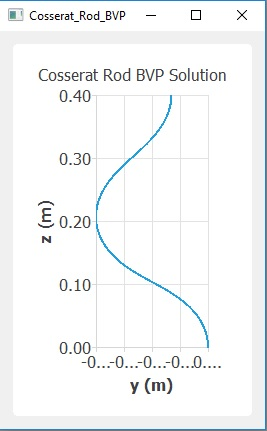
\includegraphics[width=0.4\textwidth]{fig/SolutionPlot.jpg}
	\label{fig:SolutionPlot}
\end{figure}

On a pedagogical note, there may not be a \emph{unique} solution to a BVP, but if our convex optimizer finds a zero, we have found \emph{a} solution. For instance, we would find a different solution if we set the initial guess to the following:
\begin{lstlisting}
Vector6d init_guess = Vector6d::Zero();
init_guess << 0, 4, -26, 0, 2, 0;
\end{lstlisting}
The BVP fundamentally has multiple solutions, so this would be an issue even if we weren't using the shooting method. In the context of a larger project, we would need to make sure that the solution we find is appropriate.

Another note: it would be nice from a software design standpoint to always treat a convex optimization solver as a blackbox function. However, this is generally not possible since solvers are prone to diverge or settle on non-zero local minimums. It will likely be necessary to develop a working knowledge of \emph{convex optimization} to understand a solver's behavior in more complicated use cases.
\end{document}